
%                ---- general notes    
%    p19 latex生成的文件类型介绍
%    p21 compile commands    
%       latex --> dvi + dvipdfmx ----> pdf    
%       pdflatex --> pdf    
%       xelatex  chinese
%    
%    
%%%%%%%%%%%%%%%%% article type %%%%%%%%%%%%%%%%
%\documentclass[11pt,oneside,a4paper]{article}  
\documentclass{ctexart}  


%%%%%%%%%%导言区%%%%%%%%%%%%
%%%%%mettre des "usepackage"

% 1. texdoc <pkg-name> 在终端中查看包的信息  
%    
% 2. (p20)\includeonly{<filename>} for limiting files allowed
% to be included in the file.    
%    
% 3. (p20)\syntaxonly omit .dvi .pdf, just find out erros.
%    helps accelerate compile speed    
%    
\usepackage{tabularx, makecell, multirow }
\usepackage{syntonly}
%hpyerlien
\usepackage{hyperref}
%utf8
%\usepackage[utf8]{inputenc}
%Chinese
\usepackage[]{ctex}
%to solve footnote too high 
%(this helps fix footnote to bottom of the page)
\usepackage[bottom]{footmisc}
%array: aimed at tabular
\usepackage{array}
% sanxianbiao
\usepackage{booktabs}
% graphics
\usepackage{graphicx}
% amsmath
\usepackage{amsmath}
\usepackage[]{amssymb}
%amsthm, for theorem style modification
\usepackage{amsthm}
%column seperation 
\usepackage{multicol}
%blind text
\usepackage{blindtext}
%headings and footnote
\usepackage{fancyhdr}
\pagestyle{fancy}
\fancyhf{}
\rhead{Overleaf}
\lhead{My note}
\rfoot{Page \thepage}
%color
\usepackage[]{color}
\usepackage[]{xcolor}

%%%%%%%%%%%%%%%%%%%%%%%%% new command %%%%%%%%%%%%%%%%%%%
\newcommand{\ac}[1]{\left\{ #1 \right\}}

% \usepackage{ctex}


%%%%%%%%%%导言区%%%%%%%%%%%%%
%    
%    
%---- environement:
%    \begin{<env name>}[optional]{mandatory}
%    \end{<env name>}    
%    
%---- group \command{}
%    
%    
%%%%%%%%%%%%%%%%%%%%%%%%%%%%%%%%%%%%%%%%%%%%%%%
%%%%%%%%%%  title, author, date %%%%%%%%%%%%%%%
%%%%%%%%%%%%%%%%%%%%%%%%%%%%%%%%%%%%%%%%%%%%%%%
\title{\textbf{Latex Notes}}  
\date{\today}
\author{Yuchen Hui\thanks{yuchen22314@gmail.com} 
\and Yuchen Xi\thanks{Corresponding author}}
%%%%%%%%%%%%%%%%%%%%%%%%%%%%%%%%%%%%%%%%%%%%%%%
%%%%%%%%%%%%%%%%%%%%%%%%%%%%%%%%%%%%%%%%%%%%%%%

\begin{document}
%%%%%%%%%%%%%%%%% first step : maketitle %%%%%%%%%%%%%%%%%
\maketitle

%%%%%%%%%%%%%%%%% second step : table of contents %%%%%%%%
\tableofcontents 
\listoftables
\listoffigures
\newpage
% Will make an entry for every "section" or sub-entry for subsection
\part{You mean wwwhat?}
%% Part. view pdf.
%------------------------------------------------------
%-                     Structure                      -
%------------------------------------------------------
\section[yuchen Xi]{Yuchen Hui}
      \begin{abstract}
            With de developement of Technologie. Xu jinheng 
            becomes the most powerfull man in the world.
            Savoir, c'est le pouvoir.
      \end{abstract}
      \label{se:sectionYuchen}
      % how to cut l
      \paragraph{Yuchen Hui is a stu }~{}

      \begin{verbatim}
            \section{What}
                  \begin{center}
                        What
                  \end{center}
      \end{verbatim}
      \begin{verbatim*}
            \section{What}
                  \begin{center}
                        What
                  \end{center}
      \end{verbatim*}
      \begin{enumerate}
            \item first
            \begin{itemize}
                  \item what the hell.
                  \item Yuchenchen.
                  \item[-] this is an item
                  \item[*] 
                  \begin{description}
                        \item[Lambda] lambda is a grec char. 
                        \item[Lambda] lambda is a grec char. 
                        \item[Lambda] lambda is a grec char. 
                  \end{description}
            \end{itemize}
      \end{enumerate}
      
      \begin{flushleft}
           I'm at left~~~~~~~~~~~~~~~~ 
      \end{flushleft}
      \begin{flushright}
           I'm at right \~{}\~{}\~{}\~{}\~{}\~{}\~{}
      \end{flushright}
      \begin{center}
           I'm at center \~{}\~{}\~{}\~{}\~{}\~{}\~{}
      \end{center}
      I'm tool man before quote demo. Ahhhhhhhhhhhhh
      I'm tool man before quote demo. Ahhhhhhhhhhhhh
      I'm tool man before quote demo. Ahhhhhhhhhhhhh
      I'm tool man before quote demo. Ahhhhhhhhhhhhh
      I'm tool man before quote demo. Ahhhhhhhhhhhhh
      \begin{quotation}
            hand hans lord lords.ldsjflksdjlfkjslkdj
            jlsdkfjlskdjflskdjlfjdslkfjsldkfjlsdkjfl
            lskdjflskjdflsjdlfksldkfjlsdkjflskjdflsk
            jlskdjflskdjflskjdflskjdlfskjdflksjdlfks
      \end{quotation}

      \begin{quote}
            hand hans lord lords.ldsjflksdjlfkjslkdj
            jlsdkfjlskdjflskdjlfjdslkfjsldkfjlsdkjfl
            lskdjflskjdflsjdlfksldkfjlsdkjflskjdflsk
            jlskdjflskdjflskjdflskjdlfskjdflksjdlfks
      \end{quote}
      I'm tool man After quote demo. Ahhhhhhhhhhhhh
      I'm tool man After quote demo. Ahhhhhhhhhhhhh
      I'm tool man After quote demo. Ahhhhhhhhhhhhh
      Yuchen Hui is a student 

      Yuchen Hui is 20 years old.\\
      \begin{figure}[h]
            \centering
            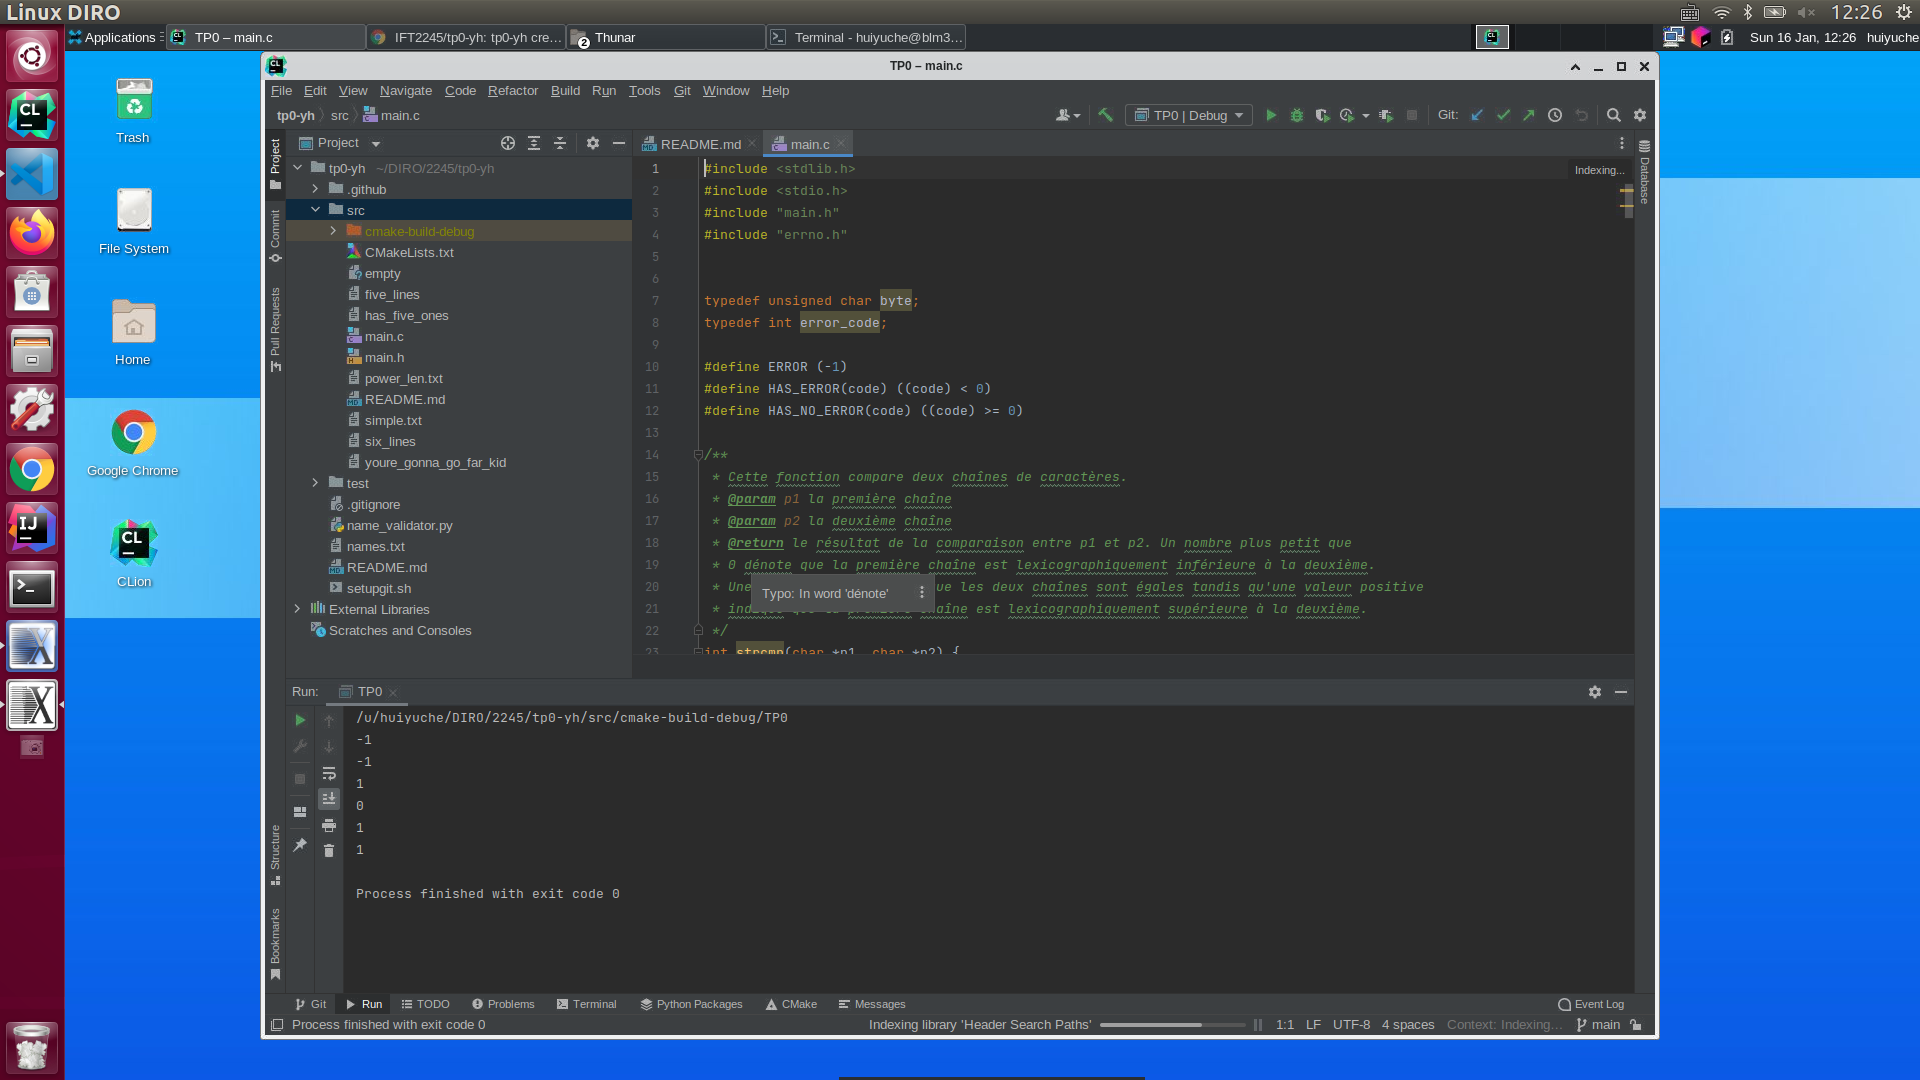
\includegraphics[scale=0.2]{linuxDirotp0.png}
            \caption{Linux DIRO Clion}
            \label{fig:linuxDIRO}
      \end{figure}
      
      \vspace{1.1em}
      \begin{tabular}[]{@{!`!`!`!`!`!`} c @{!!!!!}}
            \hline
            special leading space\footnotemark\\
            \hline
      \end{tabular}
      \footnotetext{Success this time I think.}
      \newline

      %%%%%% white line before vspace is necessary%%%%
      \vspace{1em}
      \begin{center}
            
            \begin{tabular}[]{|p{7cm}|}
            %% hline for upperline
            \hline  
            Nineteen Eighty-Four (also stylised as 1984) is a dystopian social science fiction novel and cautionary tale written by English writer George Orwell. It was published on 8 June 1949 by Secker \& Warburg as Orwell's ninth and final book completed in his lifetime. Thematically, it centres on the consequences of totalitarianism, mass surveillance and repressive regimentation of people and behaviours within societyOrwell, a democratic socialist, modelled the totalitarian government in the novel after Stalinist Russia and Nazi Germany. More broadly, the novel examines the role of truth and facts within politics and the ways in which they are manipulated. \\
            \hline
            \end{tabular}
      \end{center}

      \marginpar[]{\footnotesize margin is narrow, do not write too much.}

      \subsection{Yuchen}
            \subsubsection{Hui}
                  \label{ssse:Hui}

\part{I mean...}
\section{Text}
      \paragraph{\underline{Here is a reference to section~\ref{ssse:Hui}}}~{}\\  
            paragraph contents \\
      \emph{Here is a reference to page~\pageref{se:sectionYuchen}}\\
      Here is a test for footnote\footnote{This is a footnote. Click to come back}.\\
      Here is another test for footnote\footnote{This is a second footnote.}.
      \subsection{Latex Characters}
            %%%%%%%%%%%%%%%%%%%%%%%%%%%%%%%%%%%%%%%%%%%%%%%%%%%%%%%%%%
            %%%%%%%%%%%%%%%%%%%% Latex characters  %%%%%%%%%%%%%%%%%%%
            %%%%%%%%%%%%%%%%%%%%%%%%%%%%%%%%%%%%%%%%%%%%%%%%%%%%%%%%%%

            %   1. many space --------> one space    
            %   2. many white line -----> one white line
            %   3. \par also split paragraph   
            %   4. \\ =====> \n

            \indent Several spaces    equal one.
                  Front spaces are ignored.

            An empty line starts a new paragraph. \par
            A \verb|\par| command does the same.
            stefan monnierstefan monnierstefan monnierstefan monnierstefan monnierstefan monnierstefan monnierstefan monnierstefan monnierstefan monnierstefan monnierstefan monnierstefan monnierstefan monnier \\

            %%%%%%%%%%%%%%%%%%%%%%%%%%%%%%%%%%%%%%%
            %%          special chars            %%
            %%%%%%%%%%%%%%%%%%%%%%%%%%%%%%%%%%%%%%%
            %%    #$%&{}_^~\
            %%    we should use \# \& .... \^{} \~{} \textbackslash
            \# \& .... \^{} \~{} \textbackslash \\

            %% %%%%%%%%%%%%% how to avoid ligatures %%%%%%%%%%%%%
            %%      {}
            difficult \ldots \\
            dif{}f{}icult \ldots \\

            %%%%%%%%%%%%%%%%%%%%%%%%%%%%%%%%%%%%%%%
            %%          punctuation              %%
            %%%%%%%%%%%%%%%%%%%%%%%%%%%%%%%%%%%%%%%

            %%      1. ``''  `'
            `` Marc Feeley says `Oh Stefan je le connais...' ''\\

            %%      2. - & -- & ---   
            %%      -:composite words; 
            %%      --: number range; 
            %%      ---: po zhe hao
            daughter-in-law\\        
            pages 13--67 \\
            yes---or no?

            %%      3. \ldots == dots
            one, two, three, \dots one hundred.\\
            one, two, three, \ldots one hundred.

            %%%%%%%%%%%%%%%%%%%%%%%%%%%%%%%%%%%%%%%
            %%          francais~~~              %%
            %%%%%%%%%%%%%%%%%%%%%%%%%%%%%%%%%%%%%%%
            %%      p14, p15 img
            \'el\`eve na\"i ve !` ?` \o \oe \AE \t{oo} \textregistered \texttrademark\\

            ``Hello Wood'' \LaTeX \ \ \ \ \ son of me. \\

            %%%%%%%%%%%%%%%%%%%%%%%%%%%%%%%%%%%%%%%%%%%%%%%%%%%%%%%%%%
            %%%%%%%%%%line breaking and page breaking    %%%%%%%%%%%%%
            %%%%%%%%%%%%%%%%%%%%%%%%%%%%%%%%%%%%%%%%%%%%%%%%%%%%%%%%%%

            %%      1. tie ~~~~~~~~~~~~~~~ (fobid fenhang)
            Fig.~2a \par
            Donald ~E. Knuth \par
            %%      2. new line in the same paragraph: 
            %%         \\[<length>]  
            %%         \\*          (forbid fenye)  
            %%         \newline
            %%      3. \newpage \clearpage
            %%          双栏模式中 newpage 可以另起一栏,clearpage则是另起一页。
            %%      4. \(no)linebreak[<n>] ,\(no)pagebreak[<n>] n E [0,4] 
            %%      5. break word \-
            % \input{included.tex}
            %                   %%%%% include%%%
            % \include{included.tex}
\section{MATH}
Assume that H is a linear space with degree a. Then let \begin{align*}
	d: \mathbb{N} &\longrightarrow \mathbb{R} \\
	 n&\longmapsto d(n) = \frac{n+1}{n} 
.\end{align*}
\begin{align*}
	f: \mathbb{N} &\longrightarrow \mathbb{N} \\
	n &\longmapsto f(n) = n+1
.\end{align*}
\begin{align}
	\frac{a}{b}
	\frac{3}{4}
	\frac{4\pi_2}{5\pi_2}
	\frac{1+2+3}{2+3+4}
	\frac{4ad}{o}
	\frac{lskdfjlksdjflk}{dfd}	
	\overline{z}
\end{align}
The Pythagorean theorem is:
\begin{equation}
	a^{2}+b^{2}+c^{2} \label{pythagorean} %\notag
\end{equation}
Equation \eqref{pythagorean} is called 'gougu theorem' in Chinese.
\[
\sum\nolimits_{n=1}^{\infty} \sum_{n=h}^{\infty} a_n z^n
.\] 
In text, we can also mettre les symboles shang huozhe xia.$\sum\limits_{n=1}^{\infty} a_n z^n \sum_{n=:}^{\infty} a_n z^n$
\[
\sum_{
\begin{subarray}{c}
	1 \le i \le n\\
	j \in \mathbb{R}
\end{subarray}
}^{\infty} a_n z^n
.\] 

$\underline{\underline{\sum_{n=}^{\infty} a_n z^n}}\quad \overrightarrow{ABCDEFGH} \overrightarrow{AB}\quad \widehat{XY}$
\[
a\xleftarrow[\hat{w} hte hell]{a*b*c}bbc
.\] 
\[
.\] 
\begin{multline}
	a+b+c+d+e+f+g+h+i\\
	= j+k+l+m+n\\
	= o+p+q\\
	= w +h +t+a+t+h+e+f+u+c+k
\end{multline}
\begin{align*}
	a &= 1 & b &= 2 & c &= 3\\
	d &= 4 & e &= f & g &= 6
.\end{align*}
\begin{equation}
\begin{aligned}
	a+b+c+d+e+f+g+h+i\\
	&= j+k+l+m+n\\
	&= o+p+q\\
	&= w +h +t+a+t+h+e+f+u+c+k
\end{aligned}
\end{equation}
\[
|x|=
\begin{cases}
	-x & \text{if } x < 0,\\
	0 & if x = 0,\\
	x & if x > 0.
\end{cases}
\quad\text{and I'am the King. Who are you!!!!!!!}
.\] 

\newtheorem{nikname}{Theorem}[subsection]
\newtheorem{Nikname}{Theorem}[section]
\newtheorem*{fikname}{Theorem}
\subsection{subsection of section 3}
\begin{nikname}
	\label{thm:lignt1}
	The light speed in vacuum is $299792458\,\mathrm{m/s}$.
\end{nikname}
\begin{nikname}
	\label{thm:light2}
	The light speed in vacuum is $299792458\,\mathrm{m/s}$.
\end{nikname}
\begin{Nikname}
	\label{thm:lignt3}
	The light speed in vacuum is $299792458\,\mathrm{m/s}$.
\end{Nikname}
\begin{Nikname}
	\label{thm:light4}
	The light speed in vacuum is $299792458\,\mathrm{m/s}$.
\end{Nikname}
Where c is the light speed described in theorem \ref{thm:light4}
\theoremstyle{definition} \newtheorem{Def}{Definition}[section]
\begin{Def}
	A function is a binary relation that $\forall x \in S, \exists a $
\end{Def}
\begin{fikname}
	\label{thm:light5}
	The light speed in vacuum is $299792458\,\mathrm{m/s}$.
\end{fikname}
\section{STYLE}
\indent\tiny ajlskdjflasjflakjdslfakjslfdajslfdkjaslfdjaldskf\\
\small ablkdsjflkjd lskdjflaksjfdl alskdjflakjsf fjalksdfjaskfd.\\
\footnotesize lsakdjflakjslfajdslfjsalfdjalsjflasfajslfdasdfj.\\
\normalsize jlaskjdlfaksjlfaksddflajlskjfdlakjsdfas.\\
\large askdjflakjsdfslkdjflsssssssssssssssssssssssssssss.\\
\Large ajlskdjflaskjfdlaksjfdljsdlfakjsdlfjalfdkjalsdfjlasjfdlask.\\
\huge kdjflskjdfffffffffflskdjflsjdflkjsdlfjsldfkjlsdjflsdjfl.\\
{\Huge \underline{fldskjlfasdjflaskjdf;lakjds;lfksjd;lfkajsdlsakjfd;laksjfd;akjds;}}
< < < < < < < < < < < < < < < < < < < < < < < <
dkfjlsjfdlajsldkjflsajfdl.\\
\normalsize \indent sdkflaskfdlasdfaksjfd.
\begin{multicols}{2}
	When in Rome, do as the romans do. Here I want simply to test how latex tell
	When in Rome, do as the romans do. Here I want simply to test how latex tell
	When in Rome, do as the romans do. Here I want simply to test how latex tell
	When in Rome, do as the romans do. Here I want simply to test how latex tell
	When in Rome, do as the romans do. Here I want simply to test how latex tell
	When in Rome, do as the romans do. Here I want simply to test how latex tell
	When in Rome, do as the romans do. Here I want simply to test how latex tell a sentence or a word himself. This text is meaningless beacause of several fucking reasons. On of which is that it is meaningless. Ting jun yi xi hua, ru ting yi xi hua. As you may already noticed, there are also some chinese pinyin.
	When in Rome, do as the romans do. Here I want simply to test how latex tell a sentence or a word himself. This text is meaningless beacause of several fucking reasons. On of which is that it is meaningless. Ting jun yi xi hua, ru ting yi xi hua. As you may already noticed, there are also some chinese pinyin.
	When in Rome, do as the romans do. Here I want simply to test how latex tell a sentence or a word himself. This text is meaningless beacause of several fucking reasons. On of which is that it is meaningless. Ting jun yi xi hua, ru ting yi xi hua. As you may already noticed, there are also some chinese pinyin.
	When in Rome, do as the romans do. Here I want simply to test how latex tell a sentence or a word himself. This text is meaningless beacause of several fucking reasons. On of which is that it is meaningless. Ting jun yi xi hua, ru ting yi xi hua. As you may already noticed, there are also some chinese pinyin.
	When in Rome, do as the romans do. Here I want simply to test how latex tell a sentence or a word himself. This text is meaningless beacause of several fucking reasons. On of which is that it is meaningless. Ting jun yi xi hua, ru ting yi xi hua. As you may already noticed, there are also some chinese pinyin.
	When in Rome, do as the romans do. Here I want simply to test how latex tell a sentence or a word himself. This text is meaningless beacause of several fucking reasons. On of which is that it is meaningless. Ting jun yi xi hua, ru ting yi xi hua. As you may already noticed, there are also some chinese pinyin.
\end{multicols}
\section{\color{green}{COLOR}}
{\color{orange}Ukraine. Orange revolution. Zerinski. Putin. Vlatimil.}\\
{\color[rgb]{0.5,0.5,1}zhe shi heiheihei.}
{\color[gray]{0.5}zhe shi heiheihei.}\\
The Russian is too strong. Next, 
\textcolor{red}{Loyalty non-absolute means absolutely non-loyal.}\\

\begin{nikname}
	\colorbox[gray]{0.95}{Loyalty non-absolute means absolute disloyalty.}
\end{nikname}
|\makebox[10em][c]{mmmmmmmmmmmm}|\\
\fbox{By no means shall I love her.}
\setlength{\fboxrule}{13pt}
\setlength{\fboxsep}{1em}
\framebox[10em][c]{$\sum_{n=1}^{\infty} x^{n}$}\\
\fcolorbox{blue}{yellow}{\%\textcolor{blue}{skdjflkjsdlf}}
\textcolor{red}{Are you kidding me.}
\section{command}
你好你好。
$\ac{dkfljskdflskjlf}$
\section{Conclusion}
\begin{center} 
\end{center}
% appendix changes chapter(section) numbering to letters
\appendix
\section{appendix I}
\section{appendix II}

\end{document}
